\section{Blockdiagramm}

\begin{figure}[ht] 
\begin{center}
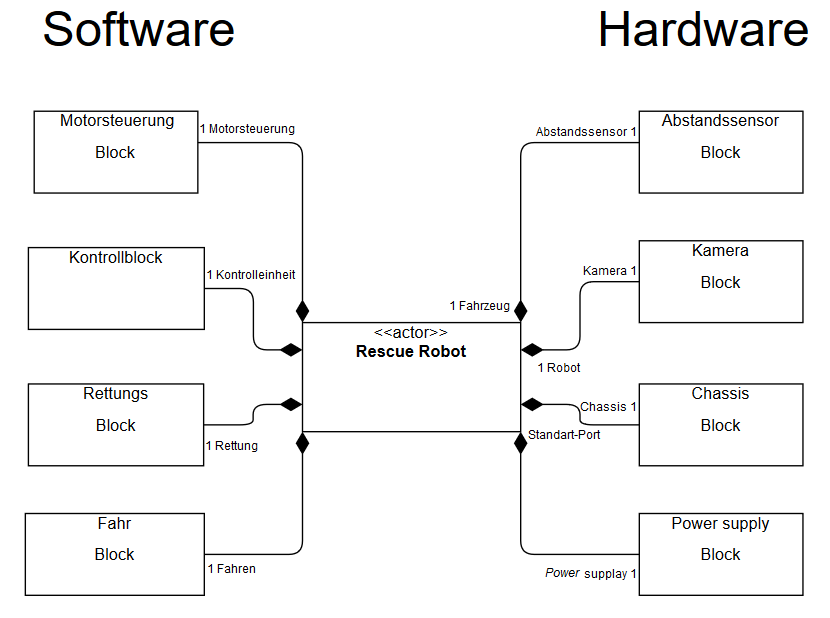
\includegraphics[width = 1\linewidth] {Blockdiagramm.png}
\caption{Blockdiagramm}
\end{center}
\end{figure}

Auf Fig. 3. wird ein Blockdiagramm dargestellt.
Mit einem Blockdiagramm werden die einzelnen Komponenten des Systems beschrieben.
Der  Hauptblock ist der Rescue Robot Block. Dieser Block ist verbunden mit den einzelnen Unterblöcken.
Die Blöcke sind aufgeteilt in Software Blöcke und Hardware Blöcke.
Zudem sind die Blöcke mit mit dem Rescue Robot Block verbunden, da diese zusammenhängend sind.